\chapter{Synthesis}
\label{synthesis}
\newpage

\section{Past}

\noindent

## Summary

This thesis can be summarized in one sentence:
we've developed the tools to measure the
error we make in phylogenetic inference and
applied it on one non-standard speciation model.
Within this chapter, I will put this into perspective.
I will first take a look at the most basic thing produced,
which is the software underlying the research,
as this is the easiest to describe objectively. 
From this rather plain foundation, I will move on 
to the way the actual research is done and ending
with the implications for the field of biology.

### Software

A simple way to quantify the amount of work
is to count the lines of code and compare with related
software. In figure \ref{fig:sloccount} I show the number of
(non-empty) lines of code for the packages I developed, the packages
I maintain, the packages I contributed to, as well as BEAST2.
BEAST2, which is the foundation of the work in this thesis, 
has the most lines of code, above 110k. After that comes
'beautier' (27k lines), phangorn (18k), 'pirouette' (17k), 'daisieme' (13k), 
DAISIE (12k) and 'razzo' (8k). 
'beautier' is an R package that creates a BEAST2 
input file, and part of the 'babette' package suite, as described
in chapter 2. 
'phangorn' is a general phylogentics package of which I fixed some bugs.
'pirouette' is the package described in chapter 3. 
'daisieme' is part of a project that did not reach fruition (see below).
DAISIE is an R package developed in our group, with 42 citations on
Google scholar. 'razzo' is the package described in chapter 4.
Summing up the packages of which I wrote most of the code, results
in 90k lines of code. This number of lines is still less than 
BEAST2 (with 110k), except all written in half the time. Also note that
BEAST2 has 26 collaborators, of which 6 contributed more than 1k lines of code.

\begin{figure}[H]
  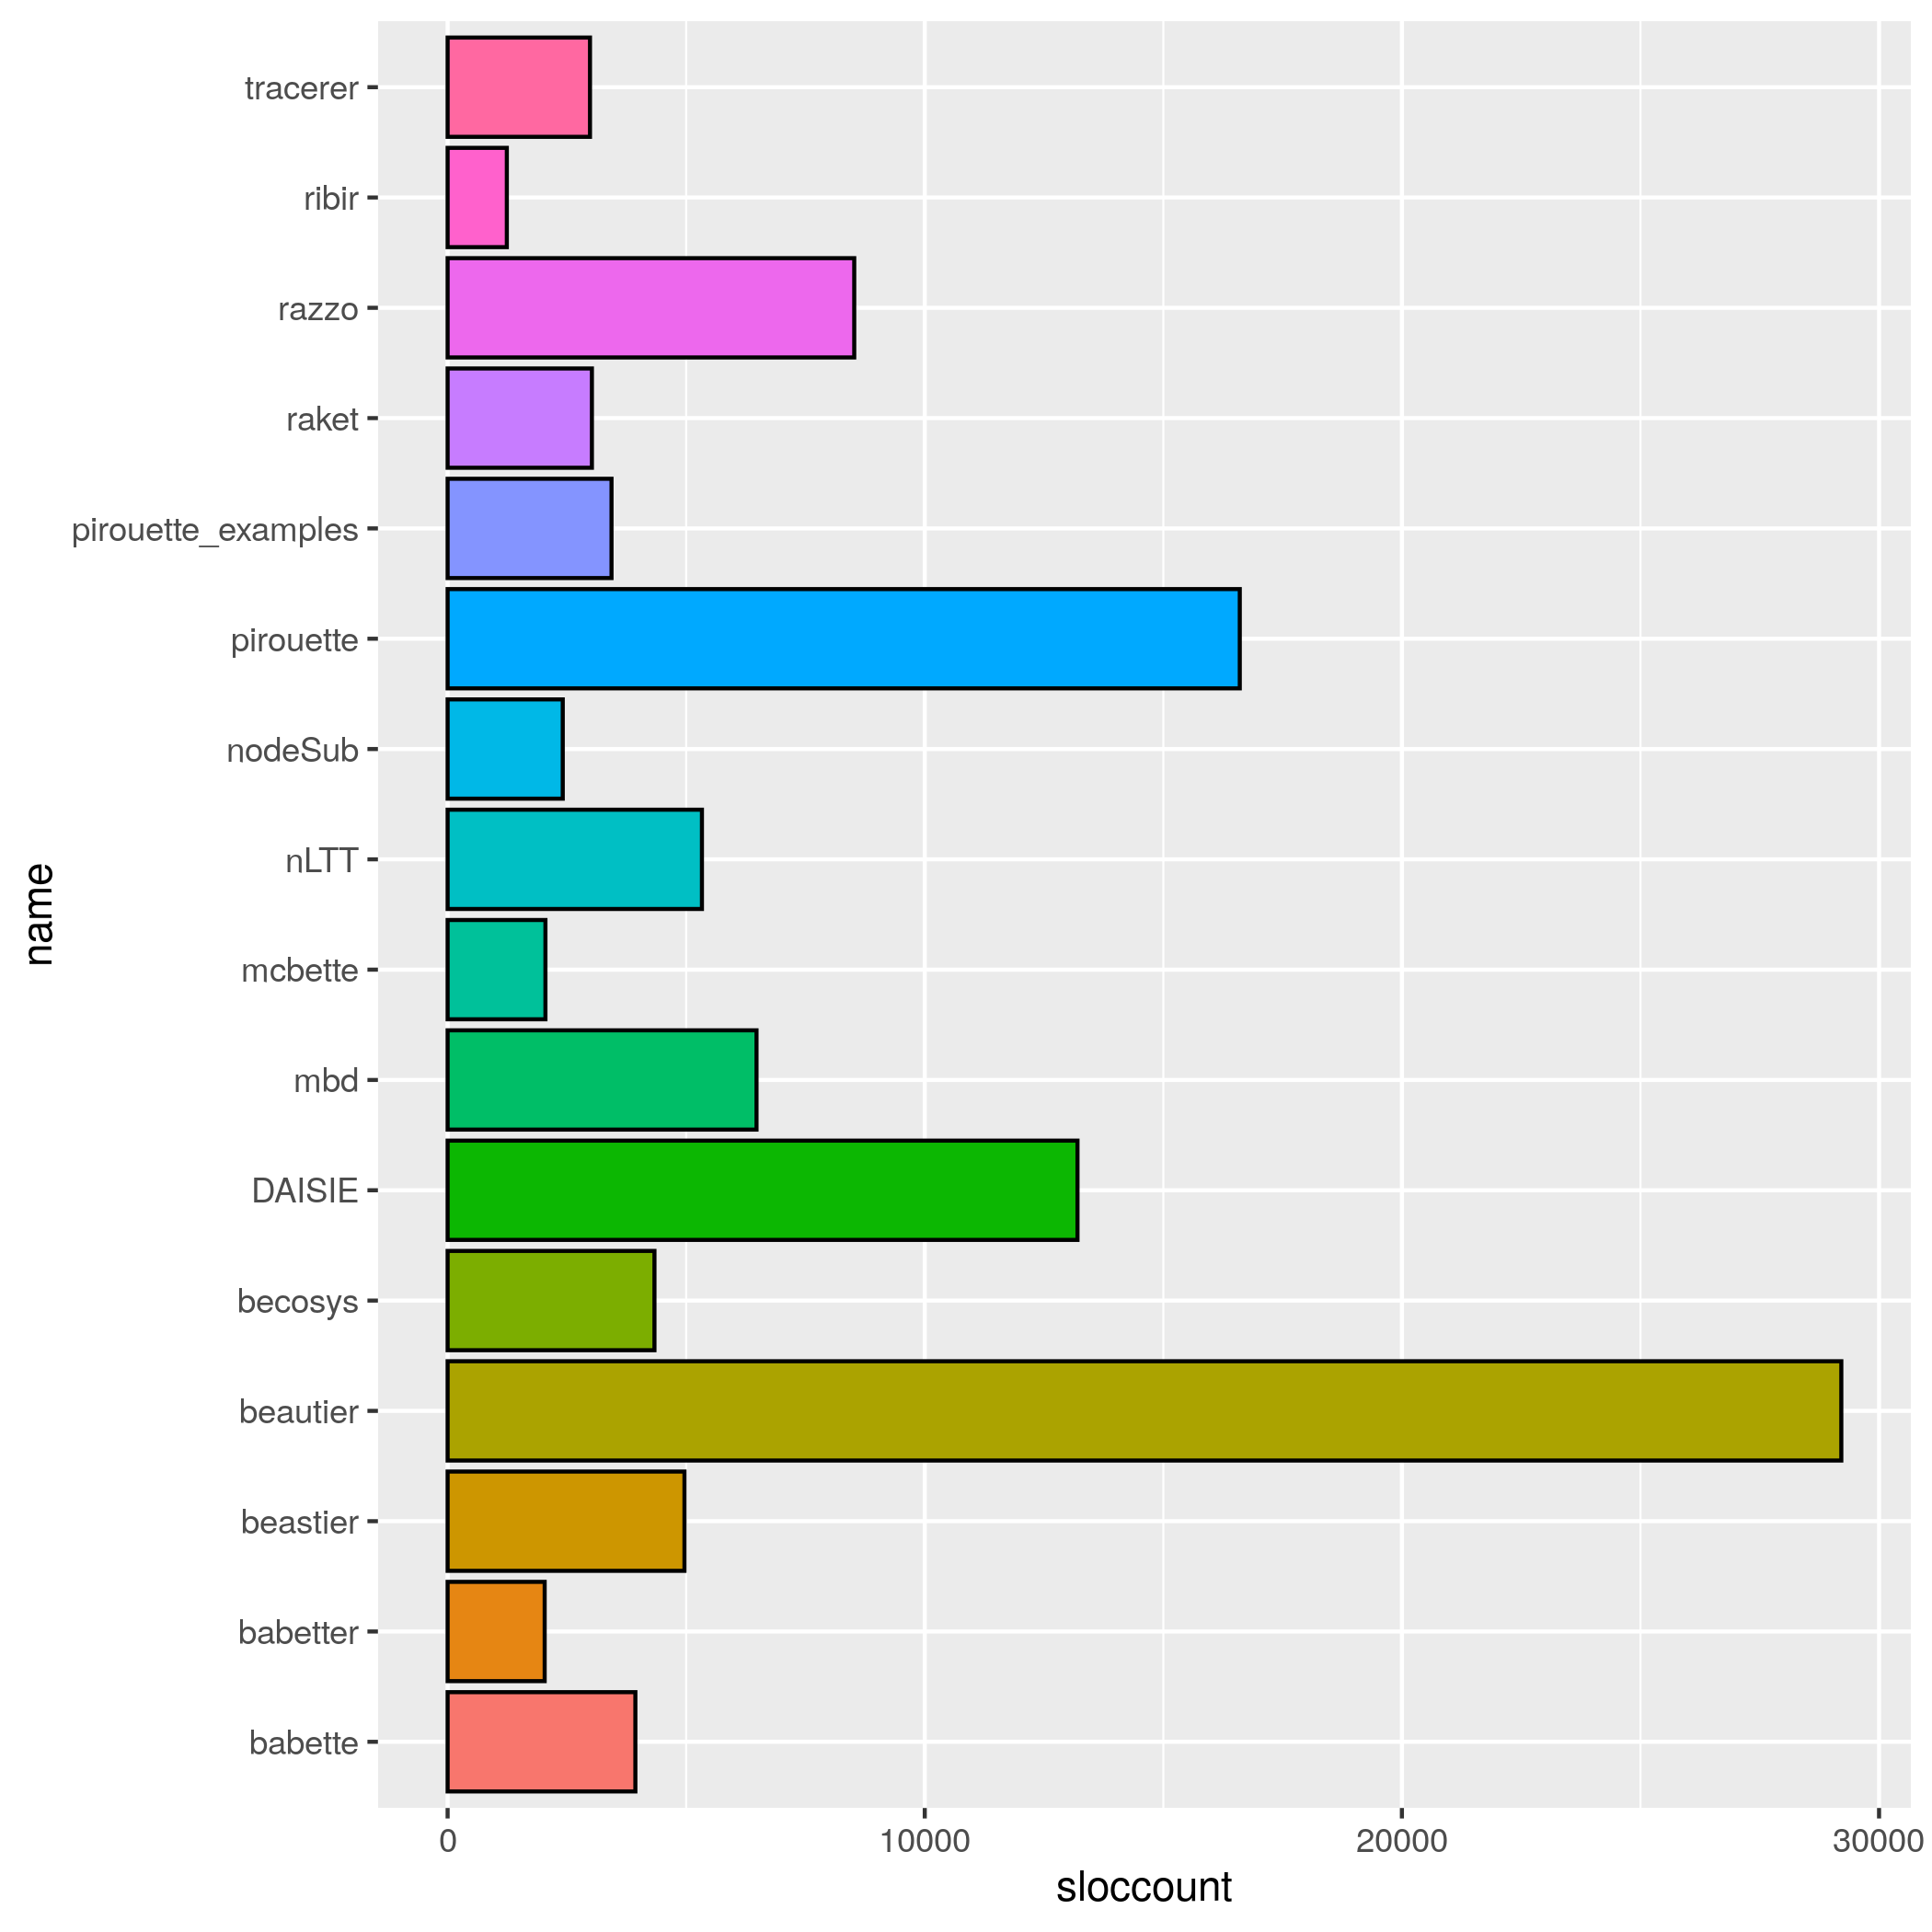
\includegraphics[width=0.8\textwidth]{sloccount.png}
  \caption{
    SLOCcount 
  }
  \label{fig:sloccount}
\end{figure}

### Quality

Judging code by the number lines of code is simple, but this is irrelevant 
to estimate the quality of the software.
Here I will highlight some indirect evidence of software quality,
for the software listed in figure \ref{fig:sloccount}.
To start with, all software in figure \ref{fig:sloccount} uses a
continuous integration (CI) service, which is known to significantly 
increase the number of bugs exposed (\cite{vasilescu2015}) and increases
the speed at which new features are added (\cite{vasilescu2015}).
A CI service is automatically activated when a developer puts a new version of
his/her software online. The CI service will create a virtual computer from
scratch, build the software and run it. These virtual computers can
be of multiple operating systems. 
Where BEAST2 and DAISIE are tested on Linux only, 'beautier',
'pirouette' and my other R packages are tested to run under MacOS and
Windows as well, assuring users of the three major operating systems
can actually run these.

A simple metric to get an idea of code quality is the code coverage.
Code coverage correlates with code quality (\cite{horgan1994,del1995correlation}). 
The code coverage is the percentage of lines
that is actually executed by tests. 
Writing tests is fundamental for writing quality code.
These tests are usually run by the CI, each time a developer puts a new version
online. Ideally all lines of code are tested. 
My software has a 100\% code coverage, compared to BEAST2, with an 
unknown/undisclosed code coverage, 'phangorn' with approximately
70\%, followed by DAISIE with approximately 60\%.

Another measure to improve code quality is peer review. Similar to
academic manuscripts, also code can be peer reviewed. 
For R code, rOpenSci is the non-profit organisation that does so.
Note that a prerequisite for a code review by rOpenSci is that code coverage is 100\%,
therefore 'phangorn' and 'DAISIE' are not yet eligible.
The five packages of the 'babette' package suite have been reviewed, 
where 'mcbette' is under review. 
The full process of the review of 'babette' took approximately one year,
as this is done in the free time of both me and the reviewers.
Mostly due to this, there has not been time yet to have 'pirouette' reviewed.

### Relevance

The relevance of software is another facet: one may write big pieces
of software of high quality, but if nobody uses it, the work is 
still irrelevant.

One way to estimate the relevance is to measure the number of CRAN downloads
per month. CRAN is a central repository for R packages, which keeps
track of the number of downloads. By this measure, in March 20202,
'phangorn' is most relevant, with 15k downloads per months, followed 
by 'beautier' (922), 'tracerer' (829) and DAISIE (740). Because BEAST2
is not an R package, it is absent from this list.

Another way to estimate the relevance is to measure the number of stars
given on GitHub. GitHub is a website that hosts source code
and that allows to develop software collaboratively.
Logged-in users (there are 40 million) can give a star to a project
to indicate his/her appreciation of the project.
Going through the projects in \ref{fig:sloccount}, most stars
are given to BEAST2: 134 (at 2020-03-09), followed
by 'phangorn' with 110 and 'babette' with 20 stars.
After 'beautier' (6), tracerer (5), beastier (5)
and mcbette (4), 'pirouette', DAISIE and nLTT only have 3 stars.
For repositories with 3 or less stars, these stars are given by
the developers themselves and thus less relevant to indicate
the relevance of a project.

## Academic relevance of software

An academic way to estimate the relevance of a piece of software,
is to count the number of citations the article describing it
has received. As of 2020-03-09 these are from Google Scholar:
BEAST2 \cite{bouckaert2014beast} has 3010 citations,
followed by phangorn \cite{schliep2011phangorn} with 1247,
DAISIE \cite{valente2014effects} has 44, 
nLTT \cite{janzen2015approximate} has 17,
and babette \cite{bilderbeek2018babette} has 2. 
Of course, older articles have had more time to accumulate citations.

## Community

A time-consuming aspects of developing software is taking care of its
users, which includes the developer(s).

Users expect that R packages are easy to install.
The R community has a centralized website from which packages
can be installed easily, called CRAN (short for 'Comprehensive R Archive 
Network').
Therefore, a developer aims to get his/her package on CRAN.
There are, however, many 
guidelines (see \url{https://cran.r-project.org/web/packages/policies.html}) before 
a package gets accepted on CRAN.
These guidelines exist to guarantee a minimum level of quality.

The most important guideline when submitting an R package to CRAN,
is that all its dependencies are on CRAN. Figure \ref{fig:dependencies}
shows the dependencies of the R packages used in this thesis, showing that
three out of the five babette packages depend on the two others. 
It would take one full year to get all packages on CRAN.

\begin{figure}[H]
  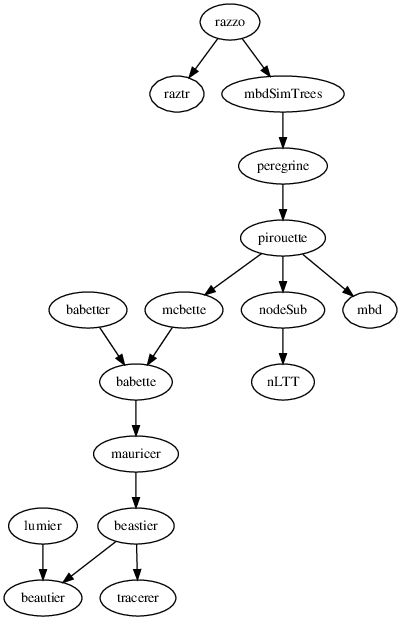
\includegraphics[width=0.8\textwidth]{dependencies.png}
  \caption{
    Minimal spanning tree of the dependencies of the R packages used in this
    thesis. Arrows go from the package dependended upon (at the tail), 
    to the package that depends on the package (at the head). For example,
    beastier depends on beautier. The packages on CRAN are beautier,
    tracerer, beastier, mauricer and babette.
  }
  \label{fig:dependencies}
\end{figure}

A consequence of taking care for the user, is that there should be
a version of each of the packages that always works, regardless of ongoing
development. If a top-level package, say 'razzo' requires some different 
functionality of a bottom-level package such as 'beautier', there
can be a cascade of new versions: a change in 'beautier' 
can cause a change in any of the packages that depend on its.
Due to this, 'beautier' (as of 2020-03-10) is at its fourth CRAN version.

Users also expect a community: a place where they can ask questions,
submit bug reports and contribute new code. 



## Scientific method

Now that we have an idea of the amount of practical work underlying
this thesis, let's take a look at the scientific methods used.

### Reproduction in practice

 * Important for science
 * Good story and significant results likelier to be published
 * Cause HARKing and p-value hacking
 * Irreproducible science

### Assuring reproduction in practice

 * Pre-registration

### Reproduction in this thesis

 * Use of dated commits
 * Wrote down hypotheses and results before having results
 * Pilot runs can be accessed, communication open

## Biology

### razzo

 * straightforward results

## Cancelled projects

### raket

 * sampling matters
 * straightforward results

### daisieme

 * straightforward results

### pbdmms

 * mechanistic models in speciation

## Future work

## Reflection

 * less features in pirouette
 * shortcut to pirouette results



 * Agree in words, less agree in deeds, less agree in others \cite{anderson2007normative}



It 



All chapters of these thesis (including this one) follow the best
practices for improving the reliability of scientific 
discoveries (\cite{munafo2017manifesto}), which are the
use of open data, software, as well as pre-registration.

\begin{figure}[H]
  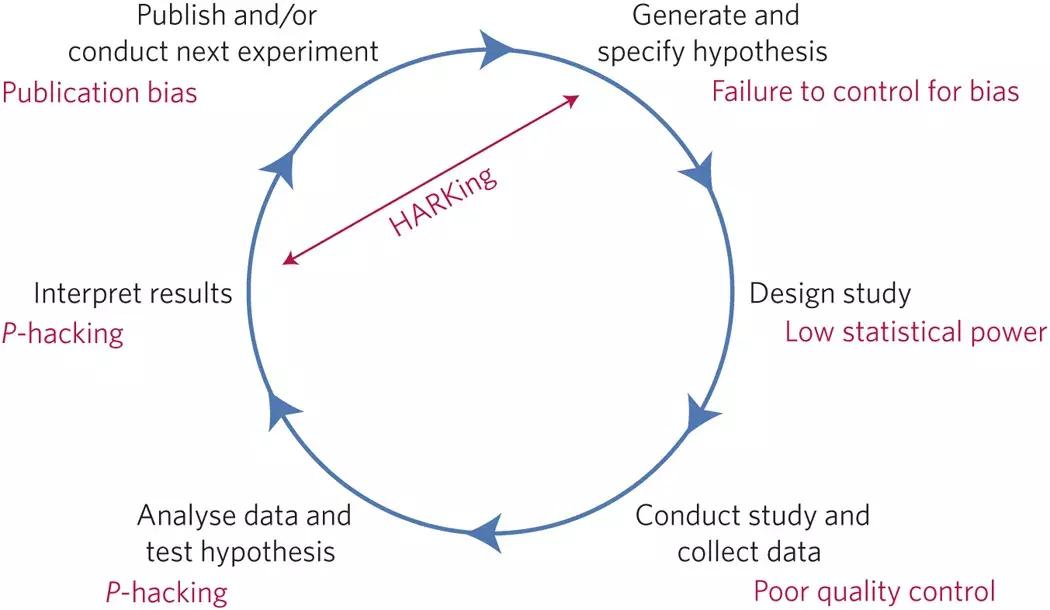
\includegraphics[width=0.8\textwidth]{munafo2017manifesto_fig_1.jpg}
  \caption{
    SLOCcount 
  }
  \label{fig:manifesto}
\end{figure}







\cite{nosek2015promoting}

The Open Science movement 
 * open publications
 * open data
 * open software
 * transparent: unability to HARK
 * reproducibility


During this PhD, I discovered the Open Science movement. 



After putting the amount of work 

It is hard to predict the relevance of the articles in this thesis.











Judging code by its quality
metrics 

 * lines of code
 * quality
 * relevance



 * tool development: babette
 * high quality
 * care for user
 * 




## Goal 

The goal of the research projects
described in this thesis
was to measure the error we make in today's phylogenetic inference.
In the end, I must conclude that the foundation to do so, is firmly 
put in place, reasonably well investigated and paves the way for
more biological example.

## Discussion of results

### pirouette and razzo only lightly explored


## Apply to PBD model: raket

## Mechanistic model: pbdmms

## Mainland extinction: daisieme

## Altmetrics

Some altmetrics:

 * 60,000 GitHub commits, 1.1k repos, 421 stars, 242 followers
 * 133 YouTube videos on babette (9), R (8), C++ (14), 68 subscribers, 11k views
 * Supervised 2 MSc students (Jorik Boer, Kees Wesselink)
 * Supervised 6 BSc students (Joris Damhuis, 
   Damian Over, Dave Nijhuis, Elles Jetten, Femke Thon, Jolien Gay)
 * Supervised 7 interns from secondary schools (Jorn Prenger, Mart Prenger, 
   Anne Hinrichs, Joshua van Waardenberg, Marijn Meerveld, Jeroen Niemendal, 
   Rijk van Putten)
 * Organised 172 social events
 * Since Jan 2017, presented 20 times at TECE
 * Publish 5 packages on CRAN (beautier, tracerer, beastier, mauricer, babette)
 * Passed rOpenSci peer-review for 4 R packages (beautier, tracerer, beastier, babette)
 * Taught +220 evenings about programming

\dropcap{T}{his} thesis answers a facet of the question 


'What is the error we make in inferring a phylogeny

describes a tool I created together with Giovanni Laudanno, 
to measure the error we make in inferring a phylogeny, due to
picking the wrong speciation model. 
With this novel tool, called \verb;pirouette; (chapter 3),
the field of phylogenetics now has a method, 
with which we demonstrate if and when the standard speciation models
are justifiably good. 

I define 'standard speciation model' as the speciation models 
present in the phylogenetic tool BEAST2, which are the Yule and
Birth-Death model. The Yule model assumes no extinction
and a constant speciation rate, where the Birth-Death model
assumes a constant speciation and extinction rate. As
it is 

There are two speciation models that are (yet) non-standard.
The first speciation model, 
unlike the standard speciation models, 
allows speciation to co-occur.
When there is a scenario in nature, in which a process triggers speciation
in multiple species, this multiple-birth death (MBD) model would be the better fit. 
In chapter 4, Giovanni Laudanno and me 
use \verb;pirouette; to 
measure the error we make, 
when we use a standard speciation model on a process we know (read: simulated) 
to follow the MBD process.
From that we found that ...

The second non-standard speciation model,
unlike the standard speciation models,
assumes that speciation takes time,
which is encorporated in the protracted-birth death (PBD) model
In chapter 5, I 
use \verb;pirouette; to 
measure the error we make, when we use a standard speciation
model on a process we know to follow the PBD process.
From that we found that ...

\section{Open questions and future work}

Now we can measure the errors we make in our phylogentic
inference, when using a standard phylogentic model on a
true process following a non-standard model. 
\verb;pirouette; can serve as a litmus test 
to measure the relevance of a novel tree prior. 

Of course, there are already ways to estimate the relevance of a
novel speciation model. A straighforward one, is to add the speciation
model to the set of standard models, after which its inference is
compared with the standard models. A drawback of this approach, is
that it is harder to develop: not only need the novel speciation model
be able to simulate its phylogenies, also a likelihood equation is needed
to allow it to be used by the phylogenetic tools. Developing such a
likelihood equation may be harder than using \verb;pirouette;.

The step forward of \verb;pirouette; is that it allows 
to quantify the error we make in our phylogentic inference, by
expressing it as (usually) two distributions: one with the baseline errors,
one with the added error caused by using an incorrect phylogenetic model.
What is missing in \verb;pirouette;, is a clear-cut interpretation of these 
error distributions, that is, a clear yes/no answer to the question: 'Is
using the standard phylogenetic models good enough?'. Only when the two
distributions overlap, can we confidently claim a yes. 

There have been defensible, yet arbitrary, choices made in the pipeline
of \verb;pirouette;. For example, a twin alignment has as much
mutations acculated from the root sequence, as the true alignment. 
This design choice should assure the Bayesian inference in the next step
to work on an equal amount of genetic information. Unknown is if this
indeed improves the judgements made by \verb;pirouette;. These choices
should one day be parameters of using \verb;pirouette; as well.

We apply the \verb;pirouette; methodology in chapter 4 and 5.
We show that the error in a Bayesian inference on
phylogenies increases when the effects of co-occuring 
or protracted speciation are stronger. 
This qualitative conclusion is obvious, 
but the extent of these errors has never been quantified before.
An obvious follow-up question is, 
what are examples in nature where we expect a high 
abundance of co-occurring or protracted speciation, 
and thus, what is the
error empiricist make?

Disregarding the results of chapters 3 and 4, there are
at least two reasons to add the MBD and PBD tree models to the standard
phylogentic models anyway. The first reason is methodological: perhaps
the \verb;pirouette; setup gave rise to an inrepresentative conclusion.
Using the actual tree prior in inference and comparing its performance
to the standard ones, is still the most straightforward way to determine,
ironically, if the novel tree prior adds value as a standard tree prior.
The second reason to add a novel tree prior the standard models, is
because of the model parameters that are estimated jointly with the
phylogenies. The clearest example is the PBD model, which allows one
to estimate biologically relevant parameters such as the duration of speciation.

This thesis gives the field of phylogenetics tools and examples of
how to quantify the effect of a tree prior on Bayesian inference.
It will help research find the border between when speciation models are
simple enough, yet not too simple. As all articles within this thesis,
this thesis itself and all its source code is free (as in freedom),
there is little in the way of this research contributing to the field. 

\references{synthesis}


RSE: De synthese is duidelijk nog niet af, dus daar zal ik niet veel over zeggen, 
behalve dat er nog in staat dat je pirouette ook op PBD hebt toegepast. 
Als dat niet in je proefschrift komt, moet je dat natuurlijk aanpassen. 
Mocht je echter pilotruns hebben gedaan, 
dan kun je die wel in de synthese of in een apart hoofdstuk kwijt. 
Dat geldt ook voor het werk aan daisieme dat je ism studenten hebt gedaan. 
Maar dat heeft geen hoge prioriteit.

Het zou ook goed zijn als je aangeeft wat precies de hordes zijn die je over 
moet bij het maken van packages als babette en pirouette. 
Ik sprak laatst iemand die dacht dat je een theoretische studie heel snel kan doen, 
alleen maar even de computer zijn gang laten gaan. 
Het is goed voor de lezer (zowel je vrienden/familie als de leescommissie) 
om inzicht te krijgen in het proces van "even de computer zijn gang laten gaan". 
Een soort "making of" dus. Als het beter past in een box of in de synthese, 
dan mag dat wat mij betreft ook.

